\documentclass[11pt]{article}

\usepackage[utf8]{inputenc}
\usepackage[T1]{fontenc}
\usepackage[spanish]{babel}
\usepackage{amsmath,amssymb}
\usepackage{booktabs}
\usepackage{graphicx}
\usepackage[margin=2.2cm]{geometry}
\usepackage{microtype}
\usepackage[hidelinks]{hyperref}

\graphicspath{{figuras/}{./}{../figuras/}}

% --- compactar un poco los flotantes y los títulos ---
\setlength{\abovecaptionskip}{4pt}
\setlength{\textfloatsep}{8pt plus 2pt minus 2pt}
\setlength{\intextsep}{8pt plus 2pt minus 2pt}
\usepackage{titlesec}
\titlespacing*{\section}{0pt}{6pt plus 1pt}{3pt}
\titlespacing*{\paragraph}{0pt}{4pt}{1em}

\title{\vspace{-1.2cm}{\Large ¿Quién gana la licitación?}\\[3pt]
\large Capacidad contra historial: rescatar a los ganadores que el baseline entierra}
\author{Grupo Valores Robados}
\date{}

\begin{document}
\maketitle
\vspace{-1.1cm}

\begin{abstract}
\noindent El baseline provisto (B0) rankea empresas por historial: quién ganó antes el mismo
trabajo, sobre todo en la misma oficina. Mostramos que eso entierra ganadores capaces que no son
``el proveedor de la casa'', y que la señal que falta está en el texto. Modelamos cada empresa como
un vector de capacidad y cada licitación como uno de requerimiento, y fusionamos esa alineación con
el historial. El modelo mejora el MRR sobre el B0 de forma significativa en 4 de 5 verticales sobre
el conjunto de prueba sellado (mejora relativa $37$--$124\,\%$), y el resultado se sostiene de
validación a prueba ($+0.074$ vs.\ $+0.073$): no es sobreajuste. El foco de este informe está en
interpretar por qué funciona y qué dicen sus parámetros.
\end{abstract}

\section{El problema y el diagnóstico}

Para cada licitación hay que rankear las empresas candidatas ($\sim$30.000 por licitación) por
probabilidad de ganarla, usando sólo información anterior a su publicación. La métrica es el MRR
(promedio de $1/\text{puesto}$ del ganador) y se compite por cuánto se mejora sobre el B0, un prior
que pondera los contratos previos de cada empresa (con decaimiento temporal) según coincidan en PSC
(qué se compra), oficina (quién compra) y NAICS. No lee texto.

\paragraph{El B0 entierra ganadores.} En validación, el B0 deja al ganador fuera del top-100 el
47\,\% de las veces; el puesto mediano del ganador es 73 sobre $\sim$32.000 candidatas. La causa es
estructural: su nivel más fuerte es ``mismo PSC $+$ misma oficina'', así que entierra a quien hizo
el mismo trabajo en otra oficina. El 61\,\% de los ganadores enterrados nunca había ganado en esa
oficina (contra 3\,\% de los que el B0 sí encuentra): no son desconocidos, simplemente no son el
proveedor habitual de esa oficina puntual. Caso típico: en ``IBM Hardware Repair'' (una base naval)
ganó una empresa de puro historial ``server maintenance'', y el B0 la mandó al puesto 4.753 por no
haberle vendido antes a esa oficina. La señal que la rescata está en el texto.

\begin{figure}[h]
  \centering
  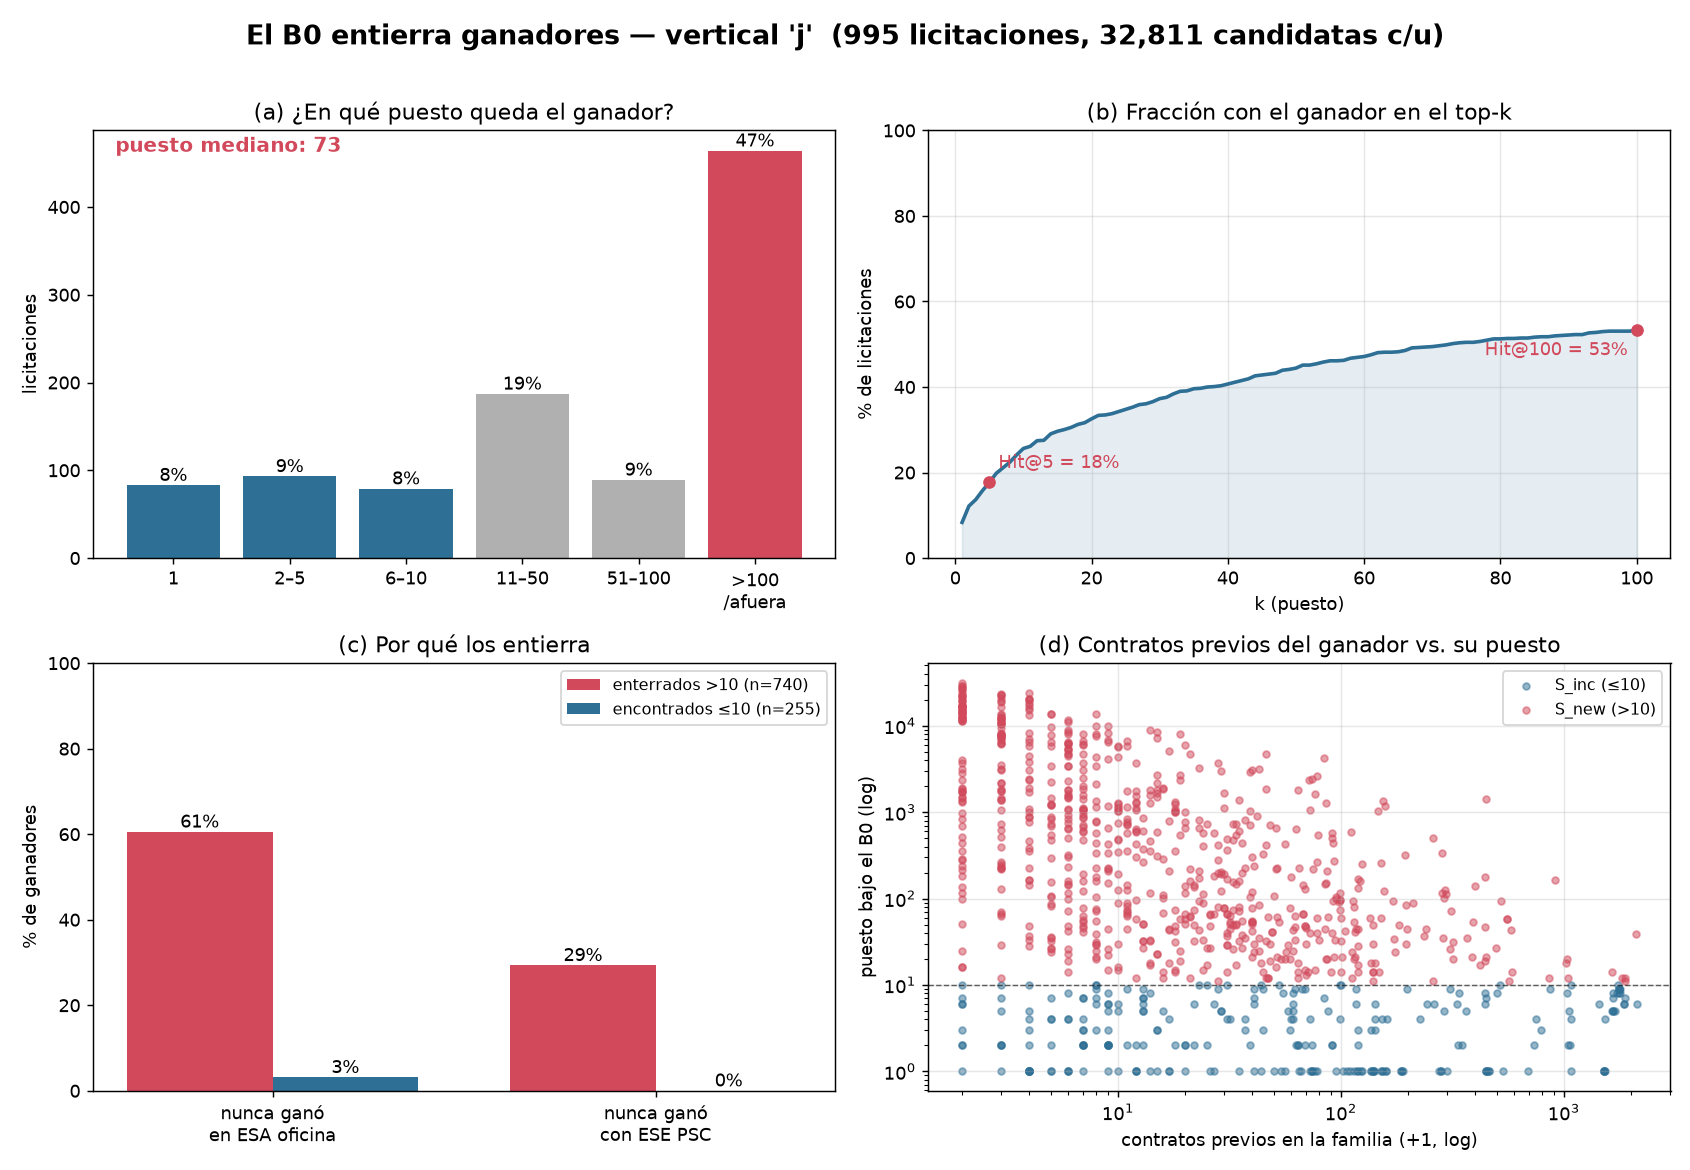
\includegraphics[width=0.78\linewidth]{b0_enterrados_j}
  \vspace{-4pt}
  \caption{(a) puesto del ganador según el B0; (b) Hit@$k$ (techo $\approx$53\,\%); (c) el 61\,\%
  de los enterrados nunca ganó en esa oficina; (d) hay ganadores con cientos de contratos previos
  igualmente enterrados: no les falta experiencia, la ganaron en otro lado.}
\end{figure}

\begin{center}\fbox{Códigos $=$ cobertura (historial). \quad Texto $=$ discriminación (capacidad).}\end{center}

\section{El modelo: capacidad contra requerimiento}

Pensamos el problema como un emparejamiento de capacidad: cada empresa $e$ es un vector de capacidad
$\mathbf{c}_e$ (qué sabe hacer) y cada licitación $q$ uno de requerimiento $\mathbf{r}_q$ (qué pide),
y puntuamos por alineación $\mathbf{c}_e\cdot\mathbf{r}_q$. Tiene una lectura de mecánica
estadística: con $P(e\text{ gana}\mid q)\propto\exp(\mathbf{c}_e\cdot\mathbf{r}_q)$ es una
distribución de Boltzmann, con el puntaje como menos la energía. Construimos ambos vectores con un
modelo de embeddings pre-entrenado (la empresa, desde el texto de sus contratos pasados; la
licitación, desde su título y las descripciones de PSC/NAICS/oficina); la similitud coseno es la
señal de capacidad. A diferencia de comparar palabras, el espacio de embeddings empareja conceptos:
``diesel generator'' y ``emergency power unit'' quedan cerca sin compartir palabras. Entre cuatro
embedders, el más chico (bge-small, 33M) fue el mejor: sobre texto corto y de dominio, los grandes
(bge-base, Gemma) agregan ruido, no señal.

Al historial le sumamos niveles de backoff (familia de PSC y jerarquía de oficina) y optimizamos
por vertical sus pesos y la vida media del decaimiento $\tau$ (B0-v2 optimizado). Reordenamos el
top-200 del B0-v2 fusionando el puesto por historial $r_{\text{hist}}$ con el puesto por capacidad
$r_{\text{cap}}$:
\[
  s(q,e)\;=\;\frac{1-\alpha}{K+r_{\text{hist}}(q,e)}\;+\;\frac{\alpha}{K+r_{\text{cap}}(q,e)},
  \qquad \alpha=0.5,\ K=5.
\]

\section{Qué significan $\alpha$ y $K$}

La fórmula es fusión de rangos (RRF): cada señal ``vota'' por una empresa con $1/(K+\text{puesto})$ y
se suman los votos. Sus dos parámetros tienen una lectura directa, y los dos óptimos son interiores
(no caen en el borde del barrido), lo que les da sentido.

\paragraph{$\alpha$: cuánto pesa la capacidad frente al historial.} $\alpha$ reparte el peso entre
las señales: $\alpha{=}0$ es B0-v2 puro (sólo historial), $\alpha{=}1$ es sólo texto. El óptimo cae
justo en $\alpha{=}0.5$: pesan igual. Que el máximo esté en el medio, y no pegado a un extremo, es
informativo --- las dos señales son igual de valiosas y no redundantes. Si el texto fuera ruido
subordinado, el óptimo estaría cerca de $0$; si el historial sobrara, cerca de $1$. Y el texto solo
($\alpha{=}1$), reemplazando al historial, empeora el ranking ($\Delta\text{MRR}=-0.037$). La
ganancia es de la sinergia: cada señal corrige los errores de la otra, no la reemplaza.

\paragraph{$K$: cuánta ventaja le da a la punta.} En $1/(K+r)$, $K$ fija cuánto más vale estar
primero que quinto. Con $K$ chico la punta manda ($K{=}0$: el puesto 1 vale el doble que el 2); con
$K$ grande los votos se aplanan y la fusión se vuelve un promedio ``democrático'' que pierde
resolución en la cabeza --- justo donde se juega el MRR. El óptimo en $K{=}5$ es el punto medio:
premia fuerte estar arriba en alguna señal, pero no tanto como para que un único puesto 1 ruidoso
arrastre todo. Equilibra confianza en la punta contra robustez al ruido.

\paragraph{Por qué rangos y no puntajes.} Las señales viven en escalas incomparables: el B0 da una
distribución picuda (casi todo el peso en pocas empresas); el coseno es suave en $[-1,1]$. Sumar los
puntajes crudos obligaría a calibrarlos; sumar $1/(K+\text{puesto})$ usa sólo el orden, que es lo
robusto, e ignora los outliers de puntaje.

\section{Resultados e interpretación}

\begin{table}[h]
\centering
\begin{tabular}{lrccc}
\toprule
Vertical & $N$ & B0 MRR & modelo MRR & $\Delta$MRR (IC 95\%) \\
\midrule
d  & 161 & 0.090 & 0.202 & $+0.112\ (+0.068,\,+0.157)$ \\
it & 319 & 0.088 & 0.165 & $+0.077\ (+0.048,\,+0.106)$ \\
r  & 468 & 0.194 & 0.266 & $+0.071\ (+0.046,\,+0.098)$ \\
j  & 995 & 0.136 & 0.202 & $+0.067\ (+0.052,\,+0.081)$ \\
rd & 57  & 0.091 & 0.145 & $+0.054\ (-0.004,\,+0.119)$ \\
\bottomrule
\end{tabular}
\vspace{-2pt}
\caption{Modelo final (bge-small $+$ B0-v2 optimizado) sobre el conjunto de prueba sellado.
Promedio ponderado por $N$: $\Delta\text{MRR}=+0.073$.}
\end{table}

\paragraph{La mejora aparece donde el historial falla.} En relativo, el salto es mayor donde el B0
es más débil: en \texttt{d} e \texttt{it} (B0 MRR $\sim0.09$) el texto suma $+124\,\%$ y $+88\,\%$;
en \texttt{r}, donde el historial ya es fuerte (B0 MRR $0.194$), suma $+37\,\%$. Es exactamente lo
que predice la tesis: el texto rescata donde el historial no alcanza y casi no toca donde ya
acierta. Por construcción el rerank reordena dentro del shortlist del historial, así que actúa sobre
los ganadores que el B0 no ponía en la punta --- los enterrados de la Sección 1 --- sin desarmar los
que ya acertaba.

\paragraph{Por qué el MRR se mueve poco en absoluto.} El MRR pesa $1/\text{puesto}$ del ganador:
está dominado por la punta. Subir un ganador del puesto 80 al 30 casi no lo mueve; sólo suma
acercarlo al puesto 1. Por eso un $\Delta$ de $+0.07$ sobre un B0 de $\sim0.13$ es grande: no es
recall barato, es haber corrido ganadores hasta la cabeza del ranking. La contracara es que el techo
absoluto es bajo y toda ganancia se pelea en los primeros puestos.

\paragraph{No es sobreajuste.} El $\Delta$MRR ponderado pasó de $+0.074$ en validación a $+0.073$ en
prueba: idénticos. Los hiperparámetros elegidos en validación generalizan a datos que el modelo
nunca vio. (\texttt{rd} queda positivo pero no significativo: con 57 licitaciones no hay potencia
estadística, no es mala señal.)

\section{Lo que no funcionó (y por qué importa)}

\begin{itemize}\itemsep1pt
  \item Texto con TF-IDF/SVD: por debajo del B0 ($-0.006$). El salto vino de los embeddings ---
  emparejan conceptos, no palabras.
  \item Ponderación adaptativa por dificultad: variamos $\alpha$ según la ``apertura'' de cada
  licitación, medida con entropías de Rényi del historial. Ninguna de la familia superó al $\alpha$
  fijo, y la razón no es la medida sino la estructura: el texto daña tan poco los casos fáciles
  ($-0.006$) que, aun con un detector perfecto, el margen a recuperar es $\sim+0.002$, bajo el ruido.
  El peso fijo ya es casi óptimo.
  \item Reranker aprendido (regresión logística $=$ máxima entropía, y LightGBM) con muchas
  features: empató a la fusión a mano. Confirma que la combinación simple ya era casi óptima ---
  $\alpha$ y $K$ aprendidos no le ganan a $\alpha{=}0.5$, $K{=}5$.
\end{itemize}

\section{Conclusión}

El B0 entierra ganadores por premiar el historial de oficina; nuestro modelo empareja la capacidad
de cada empresa (desde el texto) con el requerimiento de cada licitación y la fusiona con el
historial, aportando justo donde el historial falla. Lo que dejan los parámetros es la lección:
$\alpha{=}0.5$ dice que texto e historial son igual de informativos y sinérgicos; $K{=}5$, que la
punta pesa pero sin dejar que un puesto ruidoso mande; y el techo de la ponderación por dificultad
es estructural, no de medida. El modelo final --- bge-small para la capacidad, B0-v2 optimizado para
el historial, y una fusión simple --- es a la vez el más preciso y el más barato de correr.

\paragraph{Créditos.} \texttt{b0.py} y \texttt{evaluar.py} fueron provistos por la cátedra; el resto
del código y los experimentos son del grupo.

\end{document}
